%\documentclass[hyperref={pdfpagelabels=false},slidetop,9pt]{beamer}
\documentclass[slidetop,8pt]{beamer}
\usepackage[T1]{fontenc}
\usepackage[utf8]{inputenc}
\newcommand{\id}{71}
\newcommand{\nom}{Théorie des mécanismes}
\newcommand{\sequence}{04}
\newcommand{\nomsequence}{Liaisons entre les solides}
\newcommand{\num}{02}
\newcommand{\type}{KH}
\newcommand{\descrip}{Liaisons équivalentes, hyperstatisme, liaisons en série et en parallèle, théorie des graphes}
\newcommand{\competences}{B2-12: Proposer une modélisation des liaisons avec leurs caractéristiques géométriques. \\ &  B2-13: Proposer un modèle cinématique paramétré à partir d'un système réel, d'une maquette numérique ou d'u \\ &  B2-17: Simplifier un modèle de mécanisme. \\ &  B2-18: Modifier un modèle pour le rendre isostatique. \\ &  C1-04: Proposer une démarche permettant d'obtenir une loi entrée-sortie géométrique.  \\ &  C2-05: Caractériser le mouvement d'un repère par rapport à un autre repère. \\ &  C2-06: Déterminer les relations entre les grandeurs géométriques ou cinématiques. }
\newcommand{\nbcomp}{7}
\newcommand{\systemes}{}
\newcommand{\systemesnum}{}
\newcommand{\systemessansaccent}{}
\newcommand{\ilot}{2}
\newcommand{\ilotstr}{02}
\newcommand{\dossierilot}{\detokenize{Ilot_02 }}

\usepackage{etex}
\usepackage{tikz}
\usepackage[european]{circuitikz}
\usepackage{pgf}
\usepackage[all]{xy}
\usepackage{pgfpages}
\usepackage{graphbox}
\usepackage{pdfpages}
%\usepackage[adobe-utopia]{mathdesign}
\usepackage{ifthen}
\usepackage{cancel}
\usepackage{framed}
\usepackage{subfig}
\usepackage{tabularx}
\usepackage{setspace}
\usepackage{soul}
\usepackage{schemabloc}
\usepackage{eqnarray}
\usepackage[dot, phantomtext]{dashundergaps}
\usepackage{media9}
\usepackage{multimedia}
\usepackage{textcomp}
\usefonttheme[onlymath]{serif}

\author{Renaud Costadoat}
\institute{Lycée Dorian}

\usepackage{multido}
\usepackage{multirow}
\usepackage{multicol} % Portions de texte en colonnes
\usepackage{flafter}%floatants après la référence

\usepackage{color}
\usepackage{xcolor}
\usepackage{colortbl}

\usepackage[gen]{eurosym}
\usepackage{tikz}
%\usepackage{pstricks,pst-node,pst-tree,pst-solides3d}
\usepackage{lmodern}
\usepackage[francais]{babel}
\usepackage{pslatex}
\usetheme{renaud}
\usepackage{times}
\usepackage[frenchmath]{newtxsf} % for sans serif symbols
\renewcommand{\familydefault}{\sfdefault}
%\usepackage{amsfonts}
%\usepackage{amsmath}
%\usepackage{mathastext}
\usepackage{verbatim}
\usepackage{moreverb}
%\usetikzlibrary{arrows,shapes}
\usepackage{graphicx}
\usepackage{psfrag}
\usepackage{wrapfig}
\usepackage{etoolbox}

\definecolor{gris25}{gray}{0.75}
\definecolor{bleu}{RGB}{18,33,98}
\definecolor{bleuf}{RGB}{42,94,171}
\definecolor{bleuc}{RGB}{231,239,247}
\definecolor{rougef}{RGB}{185,18,27}
\definecolor{rougec}{RGB}{255,188,204}%255,230,231
\definecolor{vertf}{RGB}{103,126,82}
\definecolor{vertc}{RGB}{220,255,191}

\setlength\parindent{24pt}
\parskip 7.2pt
\parindent 8pt

\newenvironment{rem}[1][\hsize]%
{%
    \def\FrameCommand
   {%
\rotatebox{90}{\textit{\textsf{Remarque}}} 
       {\color{bleuf}\vrule width 3pt}%
       \hspace{0pt}%must no space.
       \fboxsep=\FrameSep\colorbox{bleuc}%
  }%
    \MakeFramed{\hsize#1\advance\hsize-\width\FrameRestore}%
}%
{\endMakeFramed}%


\newenvironment{savoir}[1][\hsize]%
{%
    \def\FrameCommand
    {%
\rotatebox{90}{\textit{\textsf{Savoir}}} 
        {\color{bleuf}\vrule width 3pt}%
        \hspace{0pt}%must no space.
        \fboxsep=\FrameSep\colorbox{bleuc}%
    }%
    \MakeFramed{\hsize#1\advance\hsize-\width\FrameRestore}%
}%
{\endMakeFramed}%

\newenvironment{prob}[1][\hsize]%
{%
    \def\FrameCommand%
    {%
\rotatebox{90}{\textit{\textsf{Problematique}}} 
        {\color{rougef}\vrule width 3pt}%
        \hspace{0pt}%must no space.
        \fboxsep=\FrameSep\colorbox{rougec}%
    }%
    \MakeFramed{\hsize#1\advance\hsize-\width\FrameRestore}%
}%
{\endMakeFramed}%

\newenvironment{obj}[1][\hsize]%
{%
    \def\FrameCommand%
    {%
\rotatebox{90}{\textit{\textsf{Objectif}}} 
        {\color{vertf}\vrule width 3pt}%
        \hspace{0pt}%must no space.
        \fboxsep=\FrameSep\colorbox{vertc}%
    }%
    \MakeFramed{\hsize#1\advance\hsize-\width\FrameRestore}%
}%
{\endMakeFramed}%

\newenvironment{defi}[1][\hsize]%
{%
    \def\FrameCommand%
    {%
\rotatebox{90}{\textit{\textsf{Definition}}} 
        {\color{bleuf}\vrule width 3pt}%
        \hspace{0pt}%must no space.
        \fboxsep=\FrameSep\colorbox{rougec}%
    }%
    \MakeFramed{\hsize#1\advance\hsize-\width\FrameRestore}%
}%
{\endMakeFramed}%


\newenvironment{hypo}[1][\hsize]%
{%
    \def\FrameCommand%
    {%
\rotatebox{90}{\textit{\textsf{Hypothèse\\}}} 
        {\color{bleuf}\vrule width 3pt}%
        \hspace{0pt}%must no space.
        \fboxsep=\FrameSep\colorbox{bleuc}%
    }%
    \MakeFramed{\hsize#1\advance\hsize-\width\FrameRestore}%
}%
{\endMakeFramed}%


\newenvironment{prop}[1][\hsize]%
{%
    \def\FrameCommand%
    {%
\rotatebox{90}{\textit{\textsf{Propriété}}} 
        {\color{bleuf}\vrule width 3pt}%
        \hspace{0pt}%must no space.
        \fboxsep=\FrameSep\colorbox{bleuc}%
    }%
    \MakeFramed{\hsize#1\advance\hsize-\width\FrameRestore}%
}%
{\endMakeFramed}%

\newenvironment{props}[1][\hsize]%
{%
    \def\FrameCommand%
    {%
\rotatebox{90}{\textit{\textsf{Propriétés}}} 
        {\color{bleuf}\vrule width 3pt}%
        \hspace{0pt}%must no space.
        \fboxsep=\FrameSep\colorbox{bleuc}%
    }%
    \MakeFramed{\hsize#1\advance\hsize-\width\FrameRestore}%
}%
{\endMakeFramed}%

\newenvironment{exemple}[1][\hsize]%
{%
    \def\FrameCommand%
    {%
\rotatebox{90}{\textit{\textsf{Exemple}}} 
        {\color{vertf}\vrule width 3pt}%
        \hspace{0pt}%must no space.
        \fboxsep=\FrameSep\colorbox{vertc}%
    }%
    \MakeFramed{\hsize#1\advance\hsize-\width\FrameRestore}%
}%
{\endMakeFramed}%

\newenvironment{resultat}[1][\hsize]%
{%
    \def\FrameCommand%
    {%
\rotatebox{90}{\textit{\textsf{Résultat}}} 
        {\color{rougef}\vrule width 3pt}%
%        {\color{bleuf}\vrule width 3pt}%
        \hspace{0pt}%must no space.
        \fboxsep=\FrameSep\colorbox{rougec}%
    }%
    \MakeFramed{\hsize#1\advance\hsize-\width\FrameRestore}%
}%
{\endMakeFramed}%

\newenvironment{methode}[1][\hsize]%
{%
    \def\FrameCommand%
    {%
\rotatebox{90}{\textit{\textsf{Méthode\\}}} 
        {\color{rougef}\vrule width 3pt}%
        \hspace{0pt}%must no space.
        \fboxsep=\FrameSep\colorbox{rougec}%
    }%
    \MakeFramed{\hsize#1\advance\hsize-\width\FrameRestore}%
}%
{\endMakeFramed}%

\newenvironment{theo}[1][\hsize]%
{%
    \def\FrameCommand%
    {%
\rotatebox{90}{\textit{\textsf{Théorème\\}}} 
        {\color{rougef}\vrule width 3pt}%
        \hspace{0pt}%must no space.
        \fboxsep=\FrameSep\colorbox{rougec}%
    }%
    \MakeFramed{\hsize#1\advance\hsize-\width\FrameRestore}%
}%
{\endMakeFramed}%

\newenvironment{warn}[1][\hsize]%
{%
    \def\FrameCommand%
    {%
\rotatebox{90}{\textit{\textsf{Attention\\}}} 
        {\color{rougef}\vrule width 3pt}%
        \hspace{0pt}%must no space.
        \fboxsep=\FrameSep\colorbox{rougec}%
    }%
    \MakeFramed{\hsize#1\advance\hsize-\width\FrameRestore}%
}%
{\endMakeFramed}%

% \usepackage{pstricks}
%\usepackage{minitoc}
% \setcounter{minitocdepth}{4}

\setcounter{tocdepth}{2}

% \mtcselectlanguage{french} 

%\usepackage{draftcopy}% "Brouillon"
% \usepackage{floatflt}
\usepackage{psfrag}
%\usepackage{listings} % Permet d'insérer du code de programmation
\renewcommand{\baselinestretch}{1.2}

% Changer la num�rotation des figures :
% ------------------------------------
% \makeatletter
% \renewcommand{\thefigure}{\ifnum \c@section>\z@ \thesection.\fi
%  \@arabic\c@figure}
% \@addtoreset{figure}{section}
% \makeatother
 


%%%%%%%%%%%%
% Définition des vecteurs %
%%%%%%%%%%%%
 \newcommand{\vect}[1]{\overrightarrow{#1}}

%%%%%%%%%%%%
% Définition des torseusr %
%%%%%%%%%%%%

 \newcommand{\torseur}[1]{%
\left\{{#1}\right\}
}

\newcommand{\torseurcin}[3]{%
\left\{\mathcal{#1} \left(#2/#3 \right) \right\}
}

\newcommand{\torseurstat}[3]{%
\left\{\mathcal{#1} \left(#2\rightarrow #3 \right) \right\}
}

 \newcommand{\torseurc}[8]{%
%\left\{#1 \right\}=
\left\{
{#1}
\right\}
 = 
\left\{%
\begin{array}{cc}%
{#2} & {#5}\\%
{#3} & {#6}\\%
{#4} & {#7}\\%
\end{array}%
\right\}_{#8}%
}

 \newcommand{\torseurcol}[7]{
\left\{%
\begin{array}{cc}%
{#1} & {#4}\\%
{#2} & {#5}\\%
{#3} & {#6}\\%
\end{array}%
\right\}_{#7}%
}

 \newcommand{\torseurl}[3]{%
%\left\{\mathcal{#1}\right\}_{#2}=%
\left\{%
\begin{array}{l}%
{#1} \\%
{#2} %
\end{array}%
\right\}_{#3}%
}

 \newcommand{\vectv}[3]{%
\vect{V\left( {#1} \in {#2}/{#3}\right)}
}


\newcommand{\vectf}[2]{%
\vect{R\left( {#1} \rightarrow {#2}\right)}
}

\newcommand{\vectm}[3]{%
\vect{\mathcal{M}\left( {#1}, {#2} \rightarrow {#3}\right)}
}


 \newcommand{\vectg}[3]{%
\vect{\Gamma \left( {#1} \in {#2}/{#3}\right)}
}

 \newcommand{\vecto}[2]{%
\vect{\Omega\left( {#1}/{#2}\right)}
}

\newcommand{\reponse}[1][4]
{
\multido{}{#1}
{
\begin{center}
\makebox[0.9\linewidth]{\dotfill} \end{center}
}}


% }$$\left\{\mathcal{#1} \right\}_{#2} =%
% \left\{%
% \begin{array}{c}%
%  #3 \\%
%  #4 %
% \end{array}%
% \right\}_{#5}}


%  ------------------------------------------
% | Modification du formatage des sections : | 
%  ------------------------------------------

% Grands titres :
% ---------------

\newcommand{\titre}[1]{%
\begin{center}
      \bigskip
      \rule{\textwidth}{1pt}
      \par\vspace{0.1cm}
      
      \textbf{\large #1}
      \par\rule{\textwidth}{1pt}
    \end{center}
    \bigskip
  }

% Supprime le numéro du chapitre dans la numérotation des sections:
% -----------------------------------------------------------------
\makeatletter
\renewcommand{\thesection}{\@arabic\c@section}
\makeatother


% \titleformat{\chapter}[display]
% {\normalfont\Large\filcenter}
% {}
% {1pc}
% {\titlerule[1pt]
%   \vspace{1pc}%
%   \Huge}[\vspace{1ex}%
% \titlerule]


%%%% Chapitres Comme PY Pechard %%%%%%%%%
% numéro du chapitre
\DeclareFixedFont{\chapnumfont}{OT1}{phv}{b}{n}{80pt}
% pour le mot " Chapitre "
\DeclareFixedFont{\chapchapfont}{OT1}{phv}{m}{it}{40pt}
% pour le titre
\DeclareFixedFont{\chaptitfont}{T1}{phv}{b}{n}{25pt}

\definecolor{gris}{gray}{0.75}
\setbeamertemplate{section in toc}[sections numbered]

\newlength{\RoundedBoxWidth}
\newsavebox{\GrayRoundedBox}
\newenvironment{GrayBox}[1][\dimexpr\textwidth-4.5ex]%
   {\setlength{\RoundedBoxWidth}{\dimexpr#1}
    \begin{lrbox}{\GrayRoundedBox}
       \begin{minipage}{\RoundedBoxWidth}}%
   {   \end{minipage}
    \end{lrbox}
    \begin{center}
    \begin{tikzpicture}%
       \draw node[draw=bleuf,fill=bleuc,rounded corners,%
             inner sep=2ex,text width=\RoundedBoxWidth]%
             {\usebox{\GrayRoundedBox}};
    \end{tikzpicture}
    \end{center}}
    
\ifdef{\prive}{\pgfpagesuselayout{2 on 1}[a4paper,border shrink=0mm]}
\ifdef{\prive}{\setbeamertemplate{navigation symbols}{}}
\setbeamertemplate{itemize item}[ball]
%\setbeamertemplate{blocks}[rounded]%[shadow=true]
\setbeamercolor{block title}{fg=white,bg=grisf}        % titre block normal 
\setbeamercolor{block body}{fg=grisf,bg=grisc!50}      % corps block normal
\setbeamercolor{block body alerted}{fg=white,bg=warning}   % idem pour un block alerte

\title{\nom}
\date{S\sequence \ - \type\num}

\begin{document}
\shorthandoff{:!}
\bibliographystyle{abbrvnat-fr}

\usebackgroundtemplate%
{%
    \centering
\includegraphics[width=\paperwidth]{/home/renaud/Documents/Renaud/GitHub/Sciences-Ingenieur/img/fond2}%
}

{
\setbeamertemplate{navigation symbols}{}
\setbeamertemplate{headline}[pagetitre]
\setbeamertemplate{footline}[pagetitre]
\usebackgroundtemplate{\centering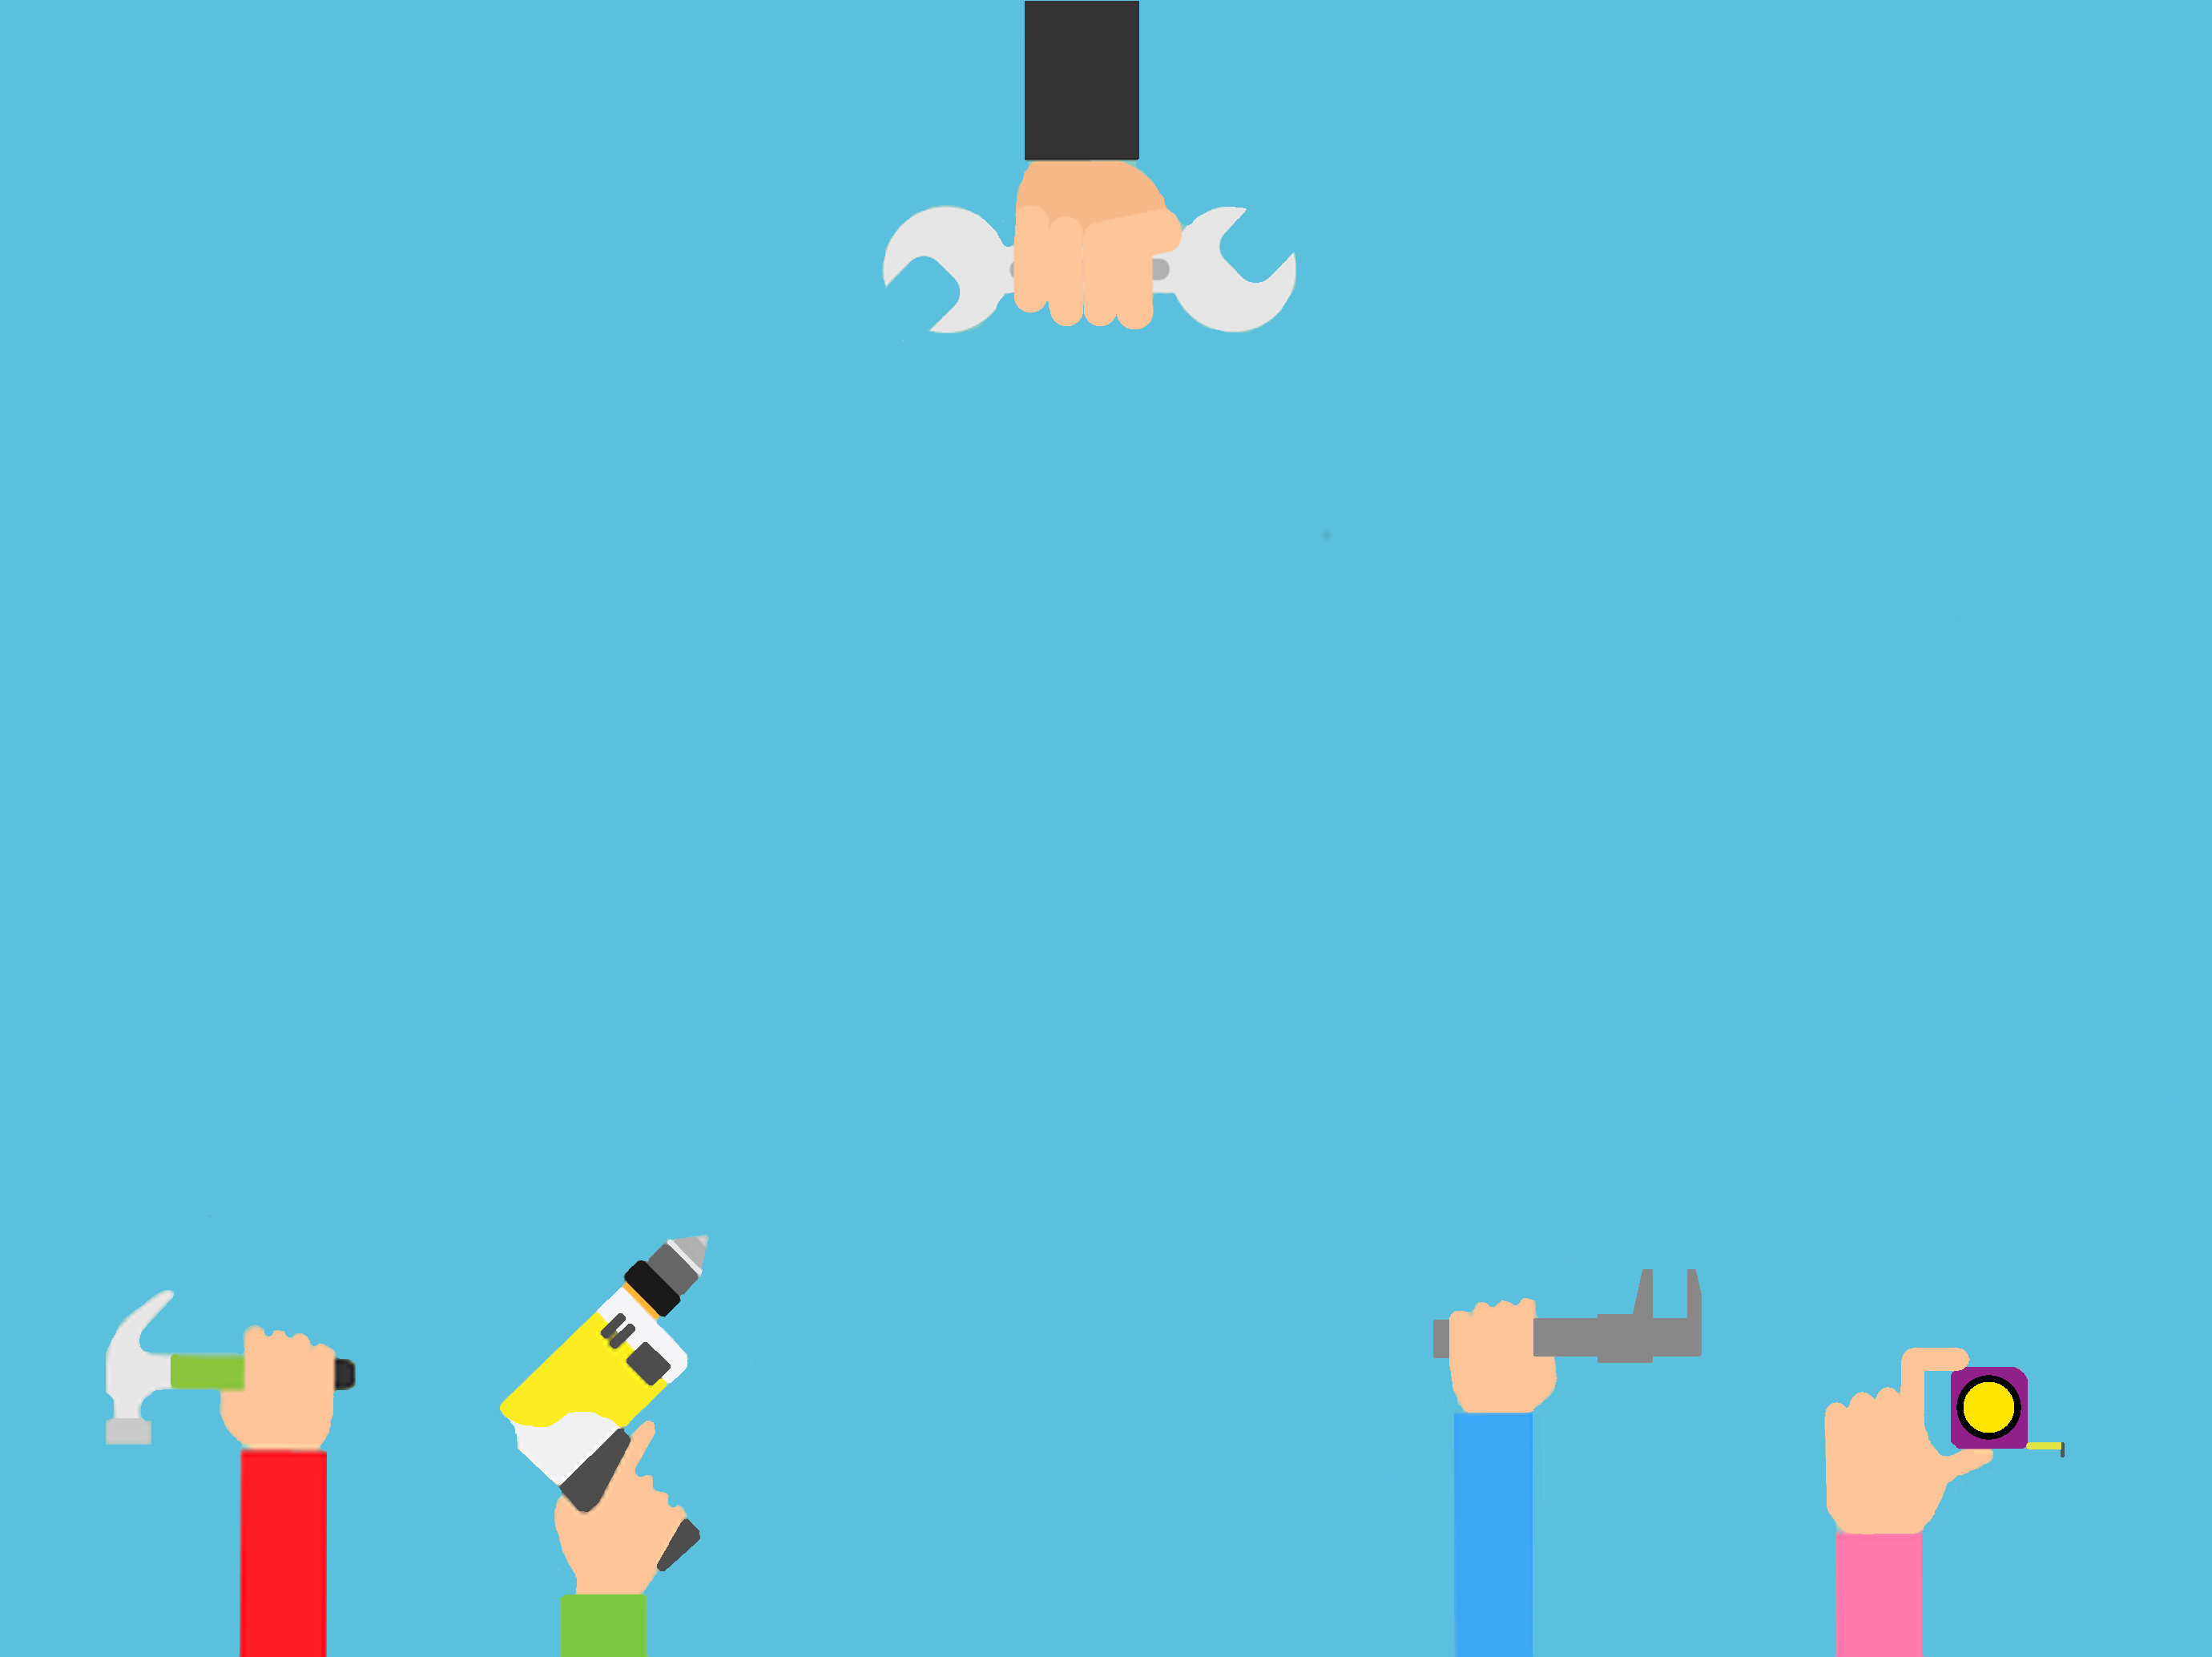
\includegraphics[width=\paperwidth]{/home/renaud/Documents/Renaud/GitHub/Sciences-Ingenieur/img/fond}}
\frame{\titlepage}
}



\section{Introduction}

{\frame{
\frametitle{Introduction}

\begin{savoir}
Vous êtes capables :
\begin{itemize}
 \item de représenter un mécanisme à l'aide d'un schéma cinématique,
 \item de le paramétrer en associant des repères à chacune des pièces,
 \item d'utiliser un modèle 3D afin de simuler le comportement d'un système. 
\end{itemize}
\end{savoir}

\begin{prob}
Vous devez êtes capables :
 \begin{itemize}
 \item de représenter n'importe quelle géométrie sur un modeleur 3D,
 \item d'assembler des pièces modélisée en les associant avec des contraintes.
 \end{itemize}
\end{prob}
}}

\section{Génération des volumes}

{\frame{
\frametitle{Génération des volumes}

\begin{savoir}
Les surfaces sont générées par l'enveloppe de toutes les positions successives d'une ligne se déplaçant suivant une autre. Celles-ci sont appelés \textbf{génératrices }.
\end{savoir}

\vfill

\begin{center}
	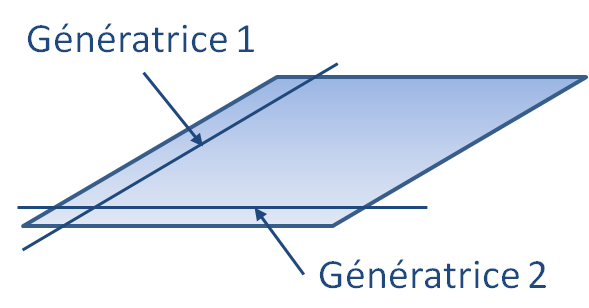
\includegraphics[width=0.4\linewidth]{img/Image1.png}
\end{center}

\vfill


A l'image des surfaces, les volumes seront créés par deux génératrices dont l'une sera non plus une ligne, mais un contour.
}}

{\frame{
\frametitle{Principaux modes de génération: Extrusion}

Il s'agit d'effectuer des translations successives d'une poli ligne fermée formant un contour, dans une direction perpendiculaire.

\vfill

\begin{center}
	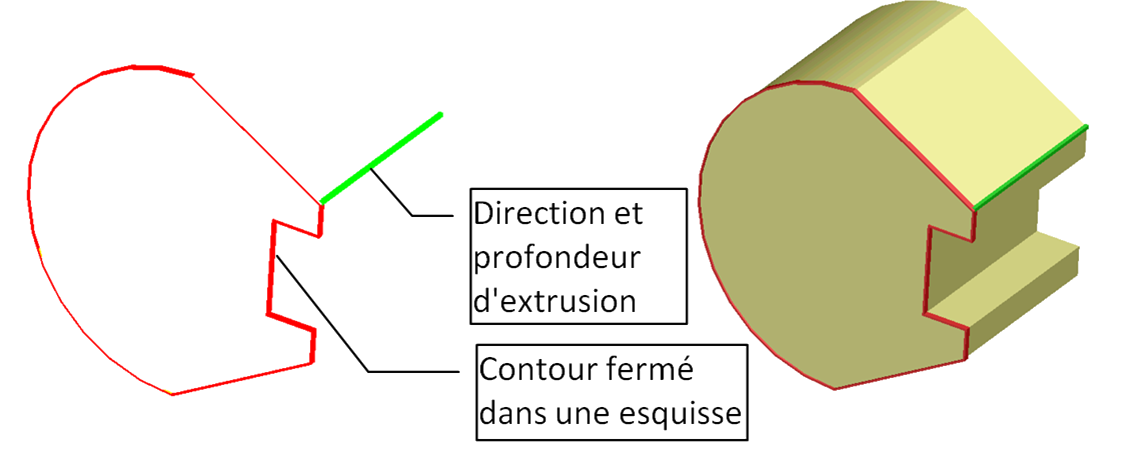
\includegraphics[width=0.9\linewidth]{img/Image2.png}
\end{center}
}}

{\frame{
\frametitle{Principaux modes de génération: Revolution}

Il s'agit d'effectuer des rotations successives d'une ligne fermée formant un contour, autour d'un axe.

\vfill

\begin{center}
	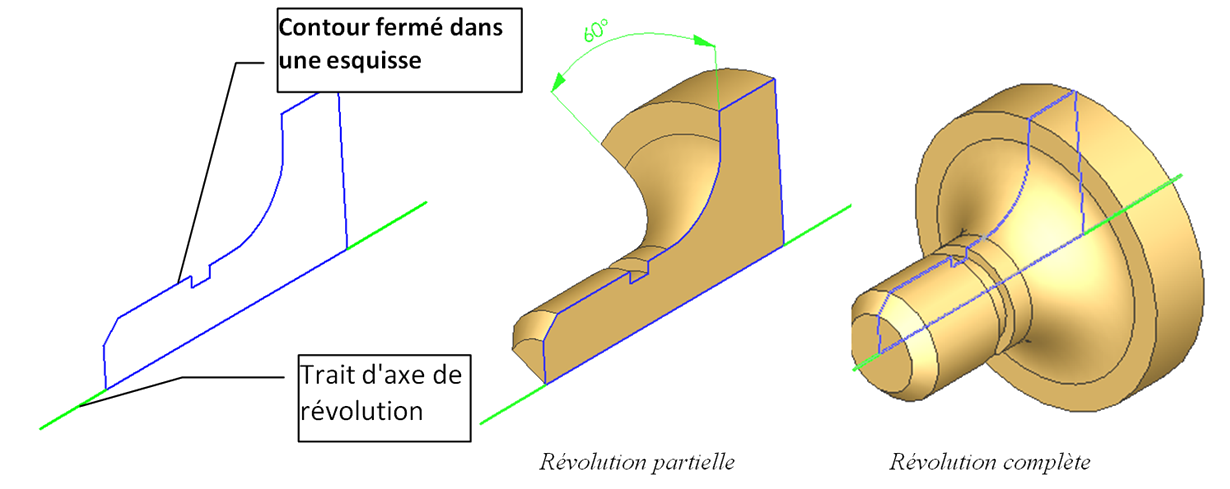
\includegraphics[width=0.9\linewidth]{img/Image3.png}
\end{center}
}}

{\frame{
\frametitle{La génération par répétition}

\begin{tabular}{c c c}
\textbf{Symétrie} & \textbf{Linéaire} & \textbf{Circulaire} \\ \\
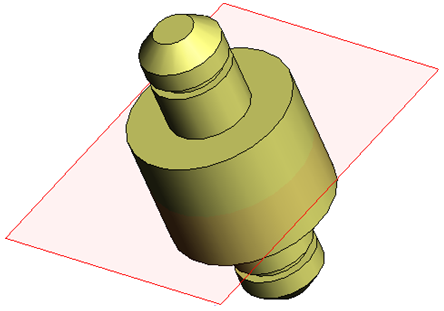
\includegraphics[width=0.3\linewidth]{img/Image4.png} & 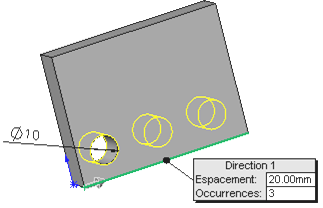
\includegraphics[width=0.3\linewidth]{img/Image5.png} & 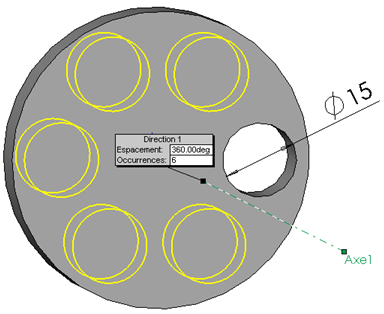
\includegraphics[width=0.3\linewidth]{img/Image6.png}
\end{tabular}
}}

{\frame{
\frametitle{Autres modes de génération: Balayage}

Il s'agit d'effectuer des déplacements successifs d'un profil (ligne fermée formant un contour), tout en suivant un chemin bien précis défini par une ligne courbe dans l'espace appelée trajectoire.

\vfill

\begin{center}
	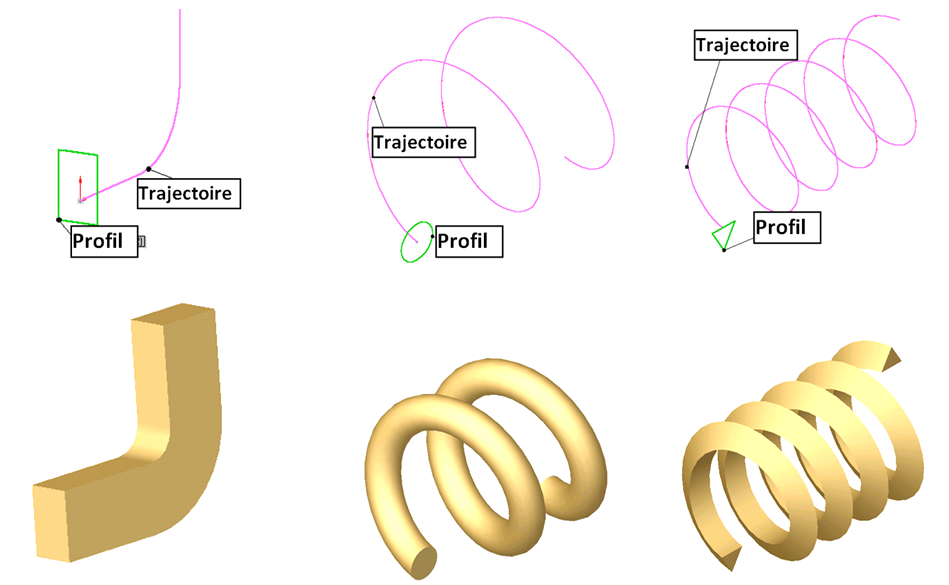
\includegraphics[width=0.8\linewidth]{img/Image7.png}
\end{center}
}}

{\frame{
\frametitle{Autres modes de génération: Lissage}

Il s'agit de relier des profils différents situés dans deux plans différents : exemple d'un volume permettant de passer d'une section carré à une section	circulaire. Les profils ne sont pas forcément reliés en ligne droite, on peut éventuellement suivre une courbe guide.

\vfill

\begin{center}
	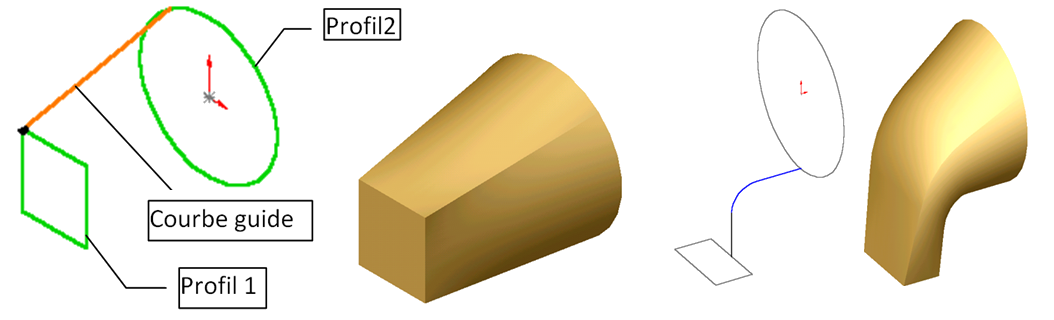
\includegraphics[width=0.9\linewidth]{img/Image8.png}
\end{center}
}}

\section{Association des différents volumes}

{\frame{
\frametitle{Association des différents volumes}

\begin{minipage}{0.55\linewidth}
\begin{itemize}
 \item Le premier volume créé dans l'arbre de création Solidworks s'appelle le \textbf{volume de base}.
 \item Ce volume s'appuie forcément sur l'un de 3 plans de base de la pièce dont l'intersection est l'origine de la pièce.
\end{itemize}
\end{minipage}
\hfill
\begin{minipage}{0.4\linewidth}
\begin{center}
	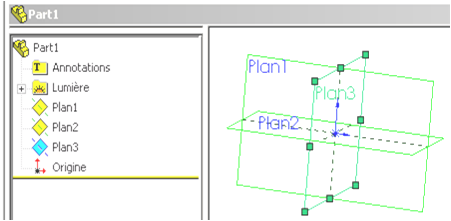
\includegraphics[width=0.9\linewidth]{img/Image9.png}
\end{center}
\end{minipage}

\vfill

\begin{itemize}
 \item Ce volume devra dans la mesure du possible être \textbf{centré sur l'origine} (les visualisations et coupes seront par la suite plus faciles).
 \item Pour cela réaliser des esquisses symétriques et construire les volumes en extrudant de chaque coté \textbf{(en plan milieu)}.
\end{itemize}
}}

{\frame{
\frametitle{Association des différents volumes}

\begin{minipage}{0.4\linewidth}
\begin{itemize}
 \item Les volumes suivants sont :
	\begin{itemize}
	 \item soit ajoutés : \textbf{bossage}
	 \item soit retranchés : \textbf{enlèvement de matière}
	\end{itemize}
 \item Paramètres contenus dans:
	\begin{itemize}
	 \item le plan d'esquisse SW : \textbf{e}
	 \item l'esquisse : \textbf{a,b,d}
	 \item la définition du volume : \textbf{c}
 	\end{itemize}
\end{itemize}

\end{minipage}
\hfill
\begin{minipage}{0.55\linewidth}
\begin{center}
	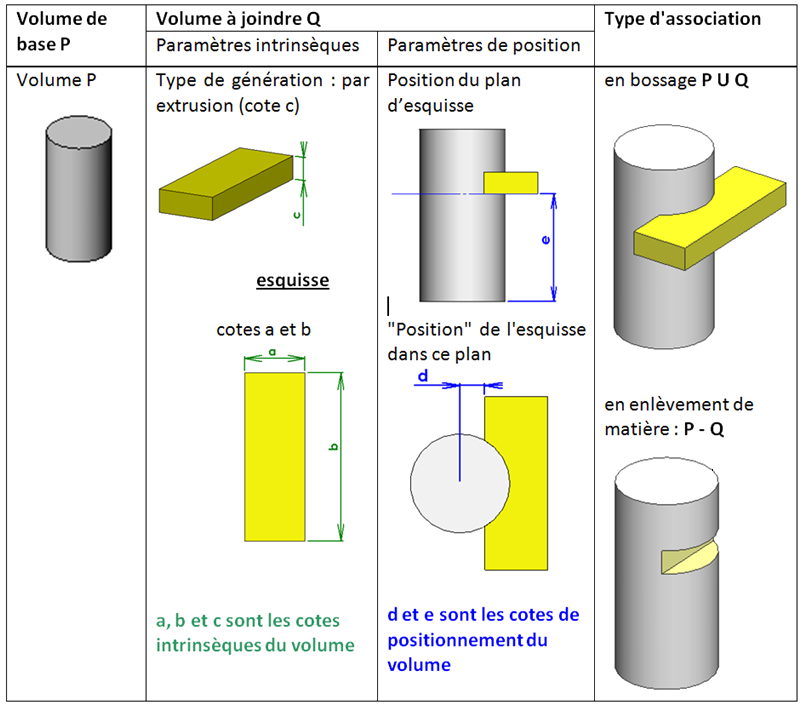
\includegraphics[width=\linewidth]{img/Image10.png}
\end{center}
\end{minipage}
}}

{\frame{
\frametitle{Arbre de construction d'une pièce}

\begin{minipage}{0.55\linewidth}
\begin{itemize}
 \item Il s'agit de définir sous forme de tableau la liste chronologique des volumes constituant la pièce :
	\begin{itemize}
	 \item Une ligne par volume.
	 \item La décomposition correspond directement à l'arbre de création feature manager de Solidworks.
	 \item La décomposition volumique doit être la plus simple possible, elle peut éventuellement correspondre directement aux opérations de fabrication successives de la pièce.
	\end{itemize}
\end{itemize}
\end{minipage}
\hfill
\begin{minipage}{0.4\linewidth}
\begin{center}
	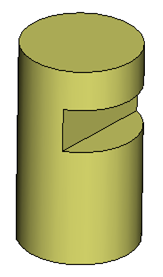
\includegraphics[width=0.3\linewidth]{img/Image11.png} \hfill
	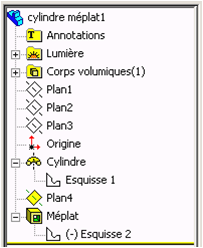
\includegraphics[width=0.55\linewidth]{img/Image12.png}
\end{center}
\end{minipage}

\vfill

\begin{itemize}
 \item La cotation des esquisses ne devra pas être surabondante, et utilisera au maximum le principe de cotation implicite.
\end{itemize}
}}

{\frame{
\frametitle{Exemple de construction d'un arbre}

\begin{minipage}{0.4\linewidth}
\begin{itemize}
 \item Contenu de l'esquisse: 
 	\begin{itemize}
	 \item formes intrinsèques des contours,
	 \item positions relatives
	\end{itemize}
 \item Paramètres volumiques:
 	\begin{itemize}
	 \item type de génération
	 \item type d'association
	 \item paramètres de génération
	 \item fonction technique associé
	\end{itemize}
\end{itemize}
\end{minipage}
\hfill
\begin{minipage}{0.55\linewidth}
\begin{center}
 \ifdef{\public}{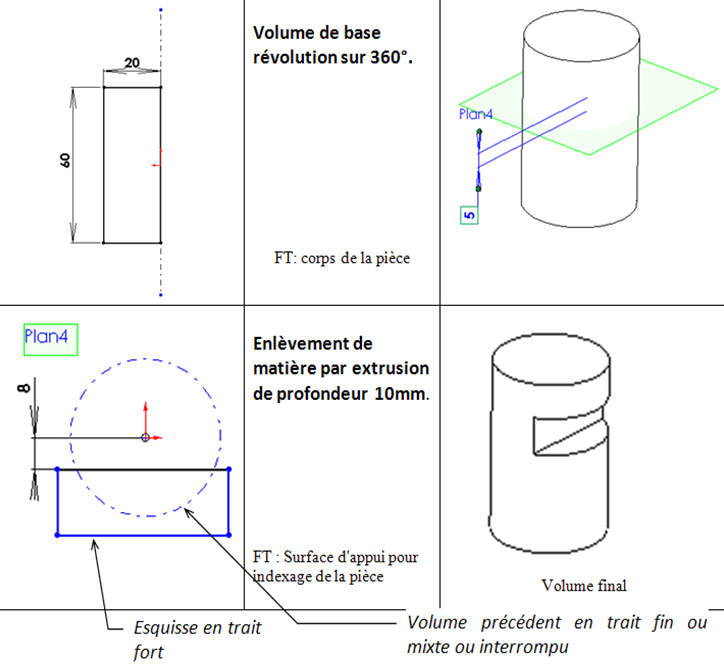
\includegraphics[width=0.9\linewidth]{img/Image13}}{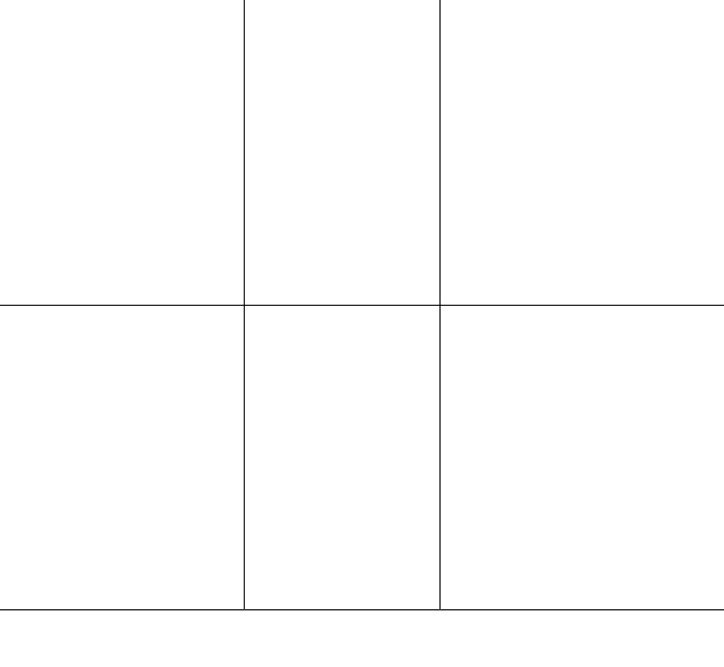
\includegraphics[width=0.9\linewidth]{img/Image13_vide}}
\end{center}
\end{minipage}

\vfill

\begin{itemize}
 \item Résultat
  \begin{itemize}
   \item représentation du volume intermédiaire obtenu en représentation « Lignes cachées », Supprimées et en noir et blanc,
   \item repérage de la position du plan d'esquisse suivante
  \end{itemize}
\end{itemize}
}}

{\frame{
\frametitle{Contraintes}

\begin{itemize}
 \item Une fois que les pièces ont été mises en forme sur le logiciel, il faut alors les mettre en places les unes par rapport aux autres.
 \item Cette mise en position s'effectue à l'aide de contraintes: 
 \begin{itemize}
 \item Distance,
 \item Coïncidence,
 \item Coaxialité,...
 \end{itemize}
\end{itemize}


\begin{rem}
 \begin{itemize}
  \item Il est absolument nécessaire d'effectuer une mise en position isostatique entre les pièces,
  \item Si le mécanisme est sur-contraint, la simulation du comportement ne pourra pas se faire correctement.
 \end{itemize}
\end{rem}
}}

{\frame{
\frametitle{Conclusion}

\begin{savoir}
Vous êtes capables :
\begin{itemize}
 \item de représenter n'importe quelle géométrie sur un modeleur 3D,
 \item d'assembler des pièces modélisée en les associant avec des contraintes.
\end{itemize}
\end{savoir}

\begin{prob}
Vous devez êtes capables d'associer à une géométrie de pièce :
 \begin{itemize}
  \item les procédés de mise en forme du brut,
  \item les opérations d'usinage permettant d'obtenir cette géométrie.
 \end{itemize} 
\end{prob}
}}


\end{document}